\chapter{Fundamentação Teórica}
\label{cap2}

\paragraph{} Neste capítulo, são introduzidos alguns conceitos chave para o entendimento do projeto. Nas próximas seções, são feitas contextualizações sobre o Mercado de Capitais, Bolsa de Valores, Ações e Aprendizado de Máquina.


\section{Mercado de Capitais, Bolsa de Valores e Ações}

\paragraph{} O Mercado de Capitais, também conhecido como Mercado de Valores Mobiliários, é um dos segmentos do sistema financeiro responsável por fazer o intermédio entre agentes superávitarios, que tem capital de investimento, e agentes deficitários, que buscam capital para rentabilizá-lo, através da compra e venda valores mobiliários (i.e., ativos financeiros) \cite{mercado_de_capitais}. Consequentemente, gera-se uma maior liquidez destes ativos e também uma melhora no fluxo de capitais entre os agentes econômicos, sejam eles os governos por meio dos bancos centrais, os bancos privados, as insituições financeiras ou até mesmo as pessoas físicas.

\paragraph{} No Brasil, o Mercado de Capitais é regulado e fiscalizado pela CVM (Comissão de Valores Mobiliários), uma autarquia federal vinculada ao Ministério da Fazenda e criada em 1976 através da Lei nº 6.385 \cite{lei_6385}.

\paragraph{} A Bolsa de Valores é uma plataforma onde se negociam os valores mobiliários do Mercado de Capitais, dentre eles ações (i.e., fatias, pedaços) de sociedades anônimas (ou companhias). No Brasil, a única Bolsa de Valores oficial existente é a B3 (Brasil, Bolsa, Balcão) \cite{b3}, que administra os sistemas de negociação, compensação, liquidação, depósito e registro para todas as principais classes de ativos.

\paragraph{} O processo de abertura de capital de uma empresa é uma iniciativa que possui vantanges estratégicas \cite{vantagens_sa} como: o aumento da confiança na perspectiva do mercado, seja para o consumidor final ou para parceiros comerciais; a solução de problemas decorrentes de processos sucessórios; e também a captação de capital de investimento, a fim de contribuir para o crescimento ou para a consolidação da companhia. Esse processo acontece através de uma oferta pública \cite{oferta_publica}, ou IPO (Initial Public Offering), onde as ações que compõe o capital social \cite{capital_social} de uma companhia são vendidas pela primeira vez ao público geral. Uma vez encerrado o IPO, estas mesmas ações passam para o mercado secundário \cite{mercado_secundario}, onde investidores as negociam entre si. Em retorno ao capital adquirido pela companhia, surgem algumas responsabilidades, dentre elas a publicação de demonstrações financeiras \cite{dem_finan}, auditadas pela própria CVM \cite{audi_dem_finan}.

\paragraph{} Para o acionista de uma sociedade anônima, existem duas formas de se obter lucro: através de proventos (dividendos e juros sobre capital próprio) \cite{proventos}; ou através de operações de compra e de venda de ações, mediante oscilações de seu valor de mercado. Conforme a expectavida corretamente induz, o lucro é comumente aferido durante a venda de um determinado papél (i.e., ação) posteriormente à sua aquisição a um preço de compra inferior. No entando, também é possível trabalhar com posições vendidas (short selling) \cite{short_selling}, onde um investidor aluga ações de outro investidor por meio de um contrato. Em seguida as vende para posteriormente recomprá-las a um preço inferior, devolvendo-as assim ao respectivo dono. Neste caso, o lucro é obtido quando expectativa de queda de um ativo se mostra verdadeira.

\subsection{Hipótese do Mercado Eficiente}

\paragraph{} A Hipótese do Mercado Eficiente, definida por FAMA \cite{fama1970efficient}, afirma que idealmente o preço de um ativo reflete toda a informação disponível sobre seu valor intrínseco. Em outras palavras, quanto menor o efeito de fatores que contribuam para uma inércia no fluxo de capital de investidores e na transmissão de informações, mais o mercado tende a ser eficiente. São estudados os três níveis de hipóteses:

\begin{itemize}
    \item HME fraca: Os preços atuais refletem o todo o histórico de informações disponibilizados publicamente.
    \item HME semi-forte: Engloba a HME fraca, acrescentando a existência de uma mudança instantânea que os preços sofrem ao surgirem novas informações.
    \item HME forte: Engloba a HME semi-forte, porém entende que a mudança instantânea dos preços acompanha toda e qualquer informação existente sobre o ativo. Assim, absolutamente nenhum investidor conseguiria obter lucro superior à média do mercado, pois não há como acessar nenhuma informação privilegiada, uma vez que ela já estaria refletido no preço corrente do ativo.
\end{itemize}

\paragraph{} O autor menciona que o HME forte não é estritamente válida na realidade, o que é uma afirmação coerente quando se verifica a existência de casos em que o vazamento de informações confidenciais trouxe aos acusados uma lucratividade significativa \cite{insider_trading}.

\paragraph{} A HME fraca foi verificada devido à consistência da correlação dos preços dia após dia de determinadas ações, mesmo que esta fosse baixa.

\paragraph{} A hipótese semi-forte também foi sustentada por alguns fatores, dentre eles a verificação de que os futuros pagamentos de dividendos das companhias se refletem, em média, no preços das ações \cite{fama1969adjustment}.

\paragraph{} Em resumo, o estudo das Hipóteses de Mercado Eficiente traz informações relevantes quanto se avalia a teoria por trás da possibilidade de aplicação de estratégias de trading no mercado financeiro. No entanto, é importante ressaltar que outros autores questionam ao menos parcialmente os estudos realizados por FAMA, sejam por resultados inconclusivos ou por anomalias detectadas no comportamento do mercado. Por exemplo, SHOSTAK \cite{shostak1997defense} critica abertamente a premissa de que todos os investidores teriam a mesma expectativa sobre os retornos da empresa. O ganhador do prêmio Nobel em ciências econômicas Paul Samuelson, que afirma que o a HME funciona muito melhor para ações individuais do que para o mercado como um todo \cite{jung2005samuelson}. Já o investidor Jack Schwager afirma que a HME está correta pelos motivos errados \cite{schwager2012market}, pois é muito difícil bater a média do mercado de forma consistente ao mesmo tempo que investidores possuem habilidades diferentes, portanto a informação não é interpretada e aplicada por todos da mesma forma.


\subsection{Índice de Bolsa de Valores}

Índices de Bolsas de Valores \cite{stock_index} são métricas criadas para avaliar a saúde de um determinado grupo de ações negociadas na bolsa. Cada índice possui uma regra própria de criação que define quais ações são englobadas e com quais pesos, como por exemplo:

\begin{itemize}
    \item S\&P 500: Um dos mais conhecidos no mercado. É a média ponderada pelo capital social das 500 maiores companhias do mercado americano.
    \item Dow Jones Industrial Average: É a média ponderada pelo preço da ação das 30 maiores blue-chips industriais e financeiras do mercado americano (i.e., companhias bem conhecidas, bem estabelecidas e com grande capital social).
    \item Ibovespa: Principal indicador de desempenho do mercado brasileiro. Possui alguns critérios específicos, mas basicamente é composto pelas ações com maior volume de negociação na B3 \cite{ibovespa}.
\end{itemize}

\paragraph{} Índices não são negociáveis pois não passam de métricas de mercado. Para isso existem fundos de investimentos chamados ETFs (Exchange-Traded Funds) \cite{etf}, especializados em seguir um determinado índice.

\paragraph{} No Brasil, um investidor que deseja que uma parte de seu capital acompanhe um rendimento equivalente ao iBovespa deverá investir no ETF, cujo código de negociação é BOVA11.


\subsection{Mercado Fracionário}

\paragraph{} Ações são negociadas em múltiplos de um lote, que representa uma quantidade mínima de papéis a transacionar. Nesse contexto, o Mercado Fracionário \cite{mercado_fracionario} surge com o objetivo de facilitar negiociações de volumes menores que o lote mínimo permitido. Na prática, ações fracionárias são agrupadas até formarem um lote para então serem negociadas. Normalmente o Mercado Fracionário possui menor liquidez e maior volatilidade, mas sempre acompanha o preço do ativo negociado no mercado aberto.

\paragraph{} Ações fracionárias podem ser criadas devido: a um desdobramento de ações que não gera resultado par (e.g., 3 para 2); ou a fusões e aquisições de empresas que combinam suas ações em uma razão predeterminada.

\paragraph{} Grandes investidores e fundos de investimentos não possuem problemas quanto ao capital mínimo necessário para a compra de um lote de ações, visto que negociam em quantidades muito maiores. O problema surge quando um investidor com pouco aporte financeiro deseja entrar no mercado e não consegue encontrar ativos cujo lote mínimo esteja dentro de seu orçamento.

\paragraph{} No Brasil, o lote mínimo é de 100 ações e o Mercado Fracionário permite a compra de no mínimo 1 ação.

\section{Tipos de Análises}

\subsection{Análise Fundamentalista}
\label{subsection:af}

\paragraph{} A Análise Fundamentalista (AF) é um muito utilizada para identificar tendências de flutuação no preço de ações tendo em vista um horizonte de longo prazo \cite{bulkowski2012fundamental}. Ela se baseia em fatores econômicos relacionados à companhia, como: o quadro de diretores e dirigentes maiores; o fluxo de caixa; a saúde e a situação financeira; o contexto político do país; os concorrentes de mercado; as circunstâncias climáticas; os desastres climáticos, naturais ou não, dentre outros fatores.

\paragraph{} Devido à natureza desorganizada e desestruturada dos dados que representam os fatores mencionados, torna-se muito difícil implementar uma automação.

\subsection{Análise Técnica}
\label{subsection:at}

\paragraph{} A Análise Técnica (AT) busca identificar tendências de curto prazo na série temporal de preços de ações através da identificação de padrões e da criação de informações derivadas (indicadores técnicos) \cite{murphy1999technical, edwards2018technical}. Segundo a Teoria de Dow, o preço das ações é consequência de todos os acontecimentos relacionados direta ou indiretamente a uma companhia \cite{kirkpatrick2010technical}.

\paragraph{} Diferentemente da AF, a automação desta análise é muito mais fácil pois os dados normalmente são organizados e estruturados. No entanto, como são obtidos a posteriori, a dificuldade desta análise se dá na separação entre o que é ruído e o que é de fato tendência de mercado, além da criação de informações derivadas que se mostram relativamente úteis.

\paragraph{} Dentre os indicadores mais famosos e portanto utilizados, podemos citar: o volume financeiro; a identificação de tendências de alta, de baixa e de consolidação de acordo com a Teoria de Dow; as linhas de suporte e de resistência do mercado; as médias móveis; as bandas de Bollinger \cite{bollinger2002bollinger}; e o MACD (Moving Average Convergence-Divergence) \cite{appel2007understanding}.

\subsubsection*{Leitura de Gráficos de Candlesticks}

\paragraph{} Gráficos de Candlesticks\footnote{Em português: Gráfico de Velas.} são bastante utilizados na AT. A leitura é padronizada de acordo com a Figura \ref{fig:1}. Neste tipo de gráfico as cores importam, pois indicam se o balanço do período foi positivo ou negativo.

\begin{figure}[h]
    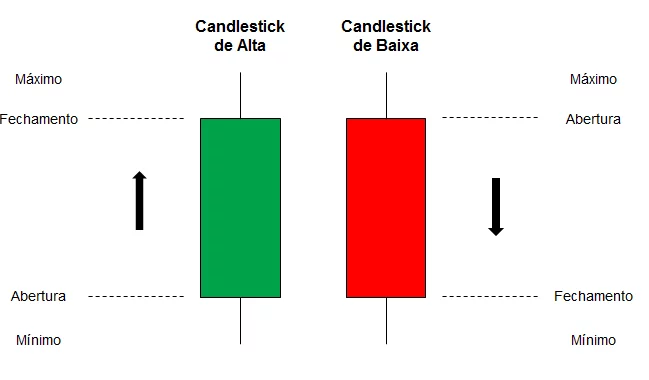
\includegraphics[scale=0.50]{candlestick.png}
    \centering
    \caption{Leitura de um gráfico de \textit{candlestick} \cite{candlestick}}
    \label{fig:1}
\end{figure}

\subsubsection*{Teoria de Dow}

\paragraph{} A Teoria de Dow, criada pelo americano Charles Henry Dow em 1884 é considerada a base da AT moderna \cite{kirkpatrick2010technical}. Embora não tivesse sido formalizada explicitamente pelo autor enquanto estava vivo, amigos e profissionais da época tiveram o trabalho de divulgar e fazer alguns ajustes. Baseada na HME, a ideia central por trás da Teoria de Dow é que a lógica econômica deve ser usada para explicar os movimentos do mercado, que em condições ideais segue o padrão de: tendência de alta\footnote{Topos e fundos ascendentes.}; topo; tendência de baixa\footnote{Topos e fundos descendentes.}; e fundo, intercalados com períodos de consolidação\footnote{Topos e fundos lateralizados.}. A Figura \ref{fig:2} ilustra esse comportamento.

\begin{figure}[h]
    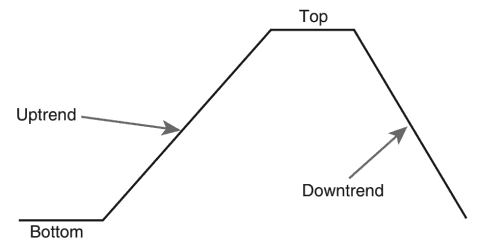
\includegraphics[scale=0.50]{dow_theory.png}
    \centering
    \caption{Comportamento do mercado ideal segundo a Teoria de Dow \cite{kirkpatrick2010technical}}
    \label{fig:2}
\end{figure}

\subsubsection*{Média Móvel Exponencial}

\paragraph{} A Média Móvel Exponencial (MME) possui uma característica que a torna relevante para estratégias de AT. Ela dá um maior peso relativo às amostras mais recentes dentro de uma série temporal. As Equações \ref{eq:2} e \ref{eq:3} mostram o seu cálculo, onde $P_t$ representa o preço atual, $\mathit{MME_{t-1}}$ é a média acumulada até o instante anterior e $K$ é uma constante definida pela quantidade de amostras desejadas $n>0$.

\begin{equation} \label{eq:2}
    \mathit{MME_t} = (P_t - \mathit{MME_{t-1}}) * K + \mathit{MME_{t-1}}
\end{equation}
\begin{equation} \label{eq:3}
    K = \frac{2}{n+1}
\end{equation}

\subsubsection*{Suporte, Resistência e Linhas de Tendência}

\paragraph{} Suporte e Resistência são regiões em um gráfico de \textit{candlestick} onde existe um grande efeito memória associado a grandes ganhos ou perdas históricas \cite{moraes2007se}. Normalmente estão associadas a eventos econômicos relevantes. A Figura \ref{fig:3} ilustra essas regiões, comumente chamadas de Linhas de Suporte e de Resistência.

\begin{figure}[h]
    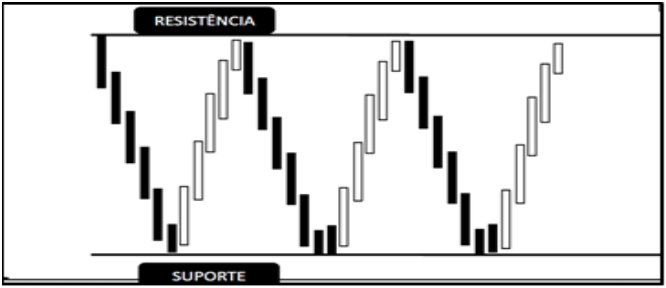
\includegraphics[scale=0.50]{suporte_resistencia.png}
    \centering
    \caption{Formação de linhas de Suporte e de Resistência \cite{moraes2007se}}
    \label{fig:3}
\end{figure}

\paragraph{} De maneira semelhante, as Linhas de Tendência oferecem uma inspeção gráfica do quanto o preço de um ativo está crescendo o diminuindo. Portanto, estão necessariamente atreladas a movimentos de tendência de alta ou de tendência de baixa. Em essência, não deixam de ser linhas se Supote e de Resistência. As Figuras \ref{fig:4} e \ref{fig:5} exemplificam esses indicadores.

\begin{figure}[h]
    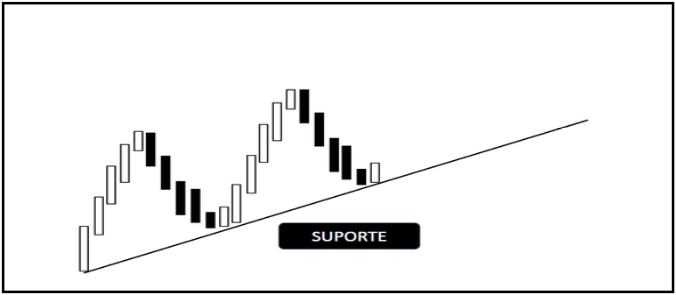
\includegraphics[scale=0.50]{lta.png}
    \centering
    \caption{Formação de uma Linha de Tendência de Alta \cite{moraes2007se}}
    \label{fig:4}
\end{figure}

\begin{figure}[h]
    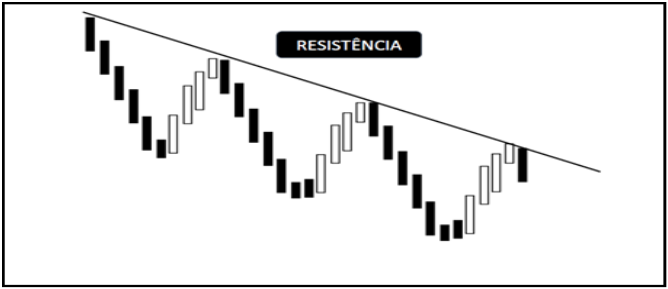
\includegraphics[scale=0.50]{ltb.png}
    \centering
    \caption{Formação de uma Linha de Tendência de Baixa \cite{moraes2007se}}
    \label{fig:5}
\end{figure}


\section{Aprendizado de Máquina}

\paragraph{} Aprendizado de Máquina (Machine Learning) é um campo de estudo dentro de Ingeligência Artificial \cite{ibm_ai} que engloba estatística e ciência da computação. O objetivo é extrair conhecimento a partir de uma conjunto de dados \cite{muller2016introduction}. A terminologia foi criada por um pesquisador da IBM chamado SAMUEL em 1959 \cite{ibm_ml} para um estudo de caso do jogo de damas \cite{arthur1959some}.

\paragraph{} Em geral, algoritmos de ML buscam realizar tarefas extremamente complexas computacionalmente sem serem explitamente programadas caso a caso. Alguns exemplos de aplicações que deixam evidente os benefícios deste método são: visão computacional, identificação de rosto, recomendação de produtos em plataformas de \textit{e-commerce}, identificação de transações financeiras fraudulentas, suporte a diagnósticos médicos, dentre diversos outros.

\paragraph{} Algoritmos de ML podem ser baseados em Aprendizado Supervisionado, Aprendizado Não Supervisionado ou até mesmo um modelo híbrido. Este trabalho utiliza apenas AS para a criação de modelos.


\subsection{Aprendizado Supervisionado}

\paragraph{} Uma das metodologias mais comuns de ML, seu objetivo é a predição de um resultado a partir de um conjunto de dados de entrada, com a condição de que o modelo tem acesso a vários exemplos de entrada e saída de dados para uma melhor performance \cite{muller2016introduction}.

\paragraph{} O conjunto de dados (\textit{dataset}) com exemplos de entrada e saída utilizado para criação do modelo é chamado de dados de treinamento (\textit{training set}). Existe um outro conjunto de dados utilzado para testar a performance do modelo. Este segundo conjunto, chamado de dados de teste (\textit{test set}), precisa ser necessariamente diferente dos dados de treinamento para evitar que o efeito memória se sobreponho à qualidade de generalização do modelo (explicado a seguir). Como regra geral de uso, é aconselhável separar 75\% dos dados para os dados de treinamento e 25\% para os dados de teste, ou algo próximo desta proporção \cite{muller2016introduction}.

\paragraph{} Todo modelo pode ser avaliado sob o ponto de vista da generalização. Essa característica indica a capacidade de realizar predições acuradas em conjuntos de dados semelhantes ao de treinamento, porém jamais vistos (dados de teste). Quanto maior a taxa de acerto nos dados de teste, melhor tende a ser a capacidade de generalização.

\paragraph{} Outras características importantes são conhecidas como \textit{overfitting} e \textit{underfitting}. Quando um modelos está muito complexo a ponto de ser sensível demais aos ruídos dos dados de treinamento, trazendo dificuldades de generalização, diz-se que ocorreu um \textit{overfitting}. De forma análoga, quando a complexidade do modelo é baixa de forma a não aproveitar devidamente as característica importantes dos dados de treinamento, implicado também em perda de generalização, diz-se que ocorreu um \textit{underfitting}. O objetivo do projetista de um modelo por AS é encontrar um ponto de equilíbrio entre essas características, chamada de ``\textit{Sweet spot}'' na Figura \ref{fig:6}, que mostra a relação entre generalização, \textit{overfitting} e \textit{underfitting}.

\begin{figure}[h]
    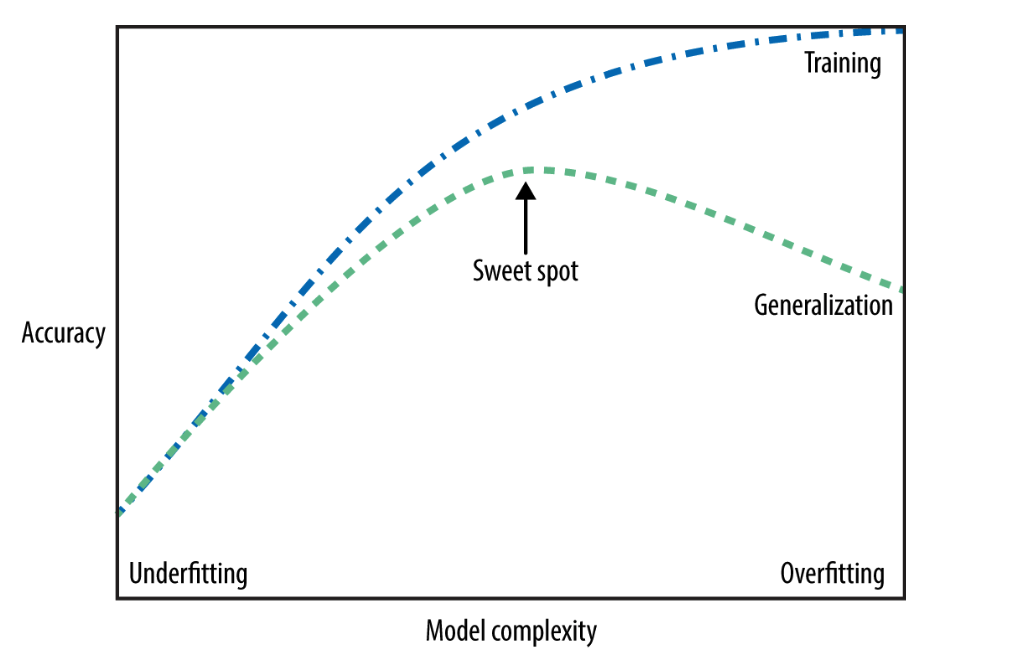
\includegraphics[scale=0.35]{generalisation.png}
    \centering
    \caption{Relação entre complexidade e acur\'acia de um modelo \cite{muller2016introduction}}
    \label{fig:6}
\end{figure}

\paragraph{} Existem dois tipos de problemas associados ao AS, os problemas de Regressão e os problemas de Classificação.


\subsection{Problema de Regressão}

\paragraph{} Este problema envolve a predição de um número contínuo a partir dos dados de entrada \cite{muller2016introduction}. Para exemplificar, pode-se citar a probabilidade de uma pessoa desenvolver uma doença auto-imune a partir de indicadores médicos específicos. Ou também um índice que traz uma espectativa de quantos kilogramas de milho serão colhidos em uma safra a partir de dados geológicos e meteorológicos.

\subsection{Problema de Classificação}

\paragraph{} Os problemas de classificação buscam escolher um rótulo (ou classe) mais provável dentre uma lista de possibilidades finitas e pré-estabelecidas \cite{muller2016introduction}. Como aplicações, pode-se citar: a previsão de escolha eleitoral de pessoas a partir de indicadores socioeconômicos; o diagnóstico de câncer em pacientes a partir de informações médicas; ou mesmo a presença e ausência de animais catalogados em um conjunto de imagens.

\paragraph{} É importante mencionar que problemas de classificação precisam de atenção ao balanceamento das classes (i.e. mesma relevância para cada classe durante o treinamento). Em outras palavras, um conjunto de dados não balanceado pode gerar um modelo pouco complexo para uma aplicação não trivial, o que implica em um ilusório indíce de acurácia nos dados de teste. Isso acontece porque o modelo tende a quase sempre escolher a classe com maior frequencia em seu treinamento, independentemente da composição dos dados. Para corrigir este efeito, deve-se deixar todas as classes com a mesma relevância durante o treinamento do modelo, o que pode ser feito através dos seguintes métodos:

\begin{itemize}
    \item \textit{Undersampling}: Diminuição de amostras pertencentes à classe mais presente. É aconselhável quando o \textit{dataset} é grande o suficiente para suportar a perda de dados sem perda significativa de generalização. Como vantagem, diminui o tempo de treinamento de um modelo. Ver Figura \ref{fig:7}.
    \item \textit{Oversampling}: Replica ou gera sinteticamente amostras pertencentes à classe menos presente. Como consequência, não há perda de informação potencialmente relevante, porém pode gerar \textit{overfitting}. Pode ser uma boa opção em \textit{datasets} pequenos \cite{weiss2007cost}. Ver Figura \ref{fig:7}.
    \item \textit{Cost Sensitive Learning} (CSL): Ao invés de alterar o tamanho do \textit{dataset}, criam-se pesos diferentes para um erro de classificação durante o treinamento. Portanto um erro numa classe menos frequente deve ser mais penalizado do que o contrário. É aconselhável em \textit{datasets} grandes ($>$ 10000) \cite{weiss2007cost}.
\end{itemize}

\begin{figure}[h]
    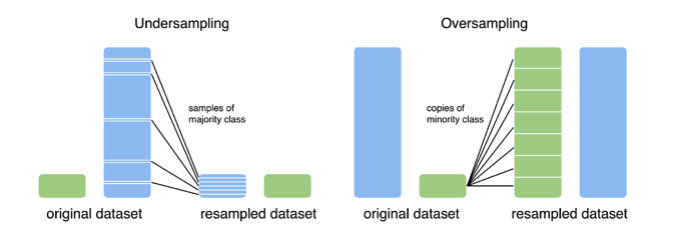
\includegraphics[scale=0.55]{over_under_sampling.png}
    \centering
    \caption{\textit{Oversampling} e \textit{Undersampling} de classes desbalanceadas \cite{over_under_sampling}}
    \label{fig:7}
\end{figure}


\subsection{Algoritmos de Aprendizado Supervisionado}

\paragraph{} Esta seção trará uma visão simplificado sobre os algoritmos de AS mais pertinentes ao presente trabalho, em ordem crescente de complexidade. O exemplos citados serão focados em problemas de classificação apenas para entendimento do raciocínio por detrás dos modelos, porém todos possuem variantes para problemas de regressão.

\subsubsection*{\textit{k-Nearest Neighbors}}

\paragraph{} k-NN é talvez o algoritmo mais simples de todos. Consiste na memorização dos dados de treinamento para predizer a classe ou o valor a partir da média dos K registros mais próximos encontrados. A Figura \ref{fig:8} mostra como funciona o critério de seleção da classe de uma amostra de teste a partir dos dados de treinamento e do parâmetro K de vizinhos selecionados.

\begin{figure}[h]
    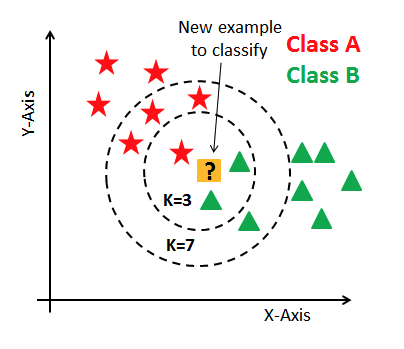
\includegraphics[scale=0.60]{knn_example.png}
    \centering
    \caption{Funcionamento de um algoritmo k-NN para o problema de classificação \cite{knn_classification}. Para K=3 a classe é B e para K=7 a classe é A.}
    \label{fig:8}
\end{figure}

\subsubsection*{\textit{Decision Tree}}

\paragraph{} Em essência, uma Árvore de Decisão\footnote{Em inglês: \textit{Decision Tree}.} é uma sequência hierárquica de estruturas de decisão \textit{if/else}\footnote{Em português: se/senão.} acerca das características do conjunto de dados. Tecnicamente, pode-se construir uma Árvore de Decisão até que todas as suas folhas\footnote{Em inglês: leafs.} estejam totalmente puras, ou seja, as sequências de decisão que levam a um resultado só englobam amostras de um tipo de classe. Ao contrário de folhas impuras, que contém a presença de mais de uma classe, onde normalmente se escolhe a de maior número de amostras como resultado. O problema é que a presença excessiva de folhas totalmente puras é acompanhado de um \textit{overfitting} do modelo, portanto precisa ser controlado. Para isso, é possível ajustar alguns parâmetros, como por exemplo: a profundidade, que define a quantidade máxima de camadas que a árvore atingirá qualquer que seja o ramo; o número mínimo de amostras para se criar uma nova ramificação; dentre outros.

\paragraph{} Algumas vantagens deste modelo estão no relativamente fácil entendimento e visualização dos critérios de decisão para o projetista em árvores pequenas. O tempo de processamento computacional envolvido na criação deste modelo é razoavelmente curto. Não é necessário um pré-processamento dos dados, uma vez que cada característica é processada separadamente. A Figura \ref{fig:9} mostra a estrutura por trás de uma Árvode de Decisão.

\begin{figure}[h]
    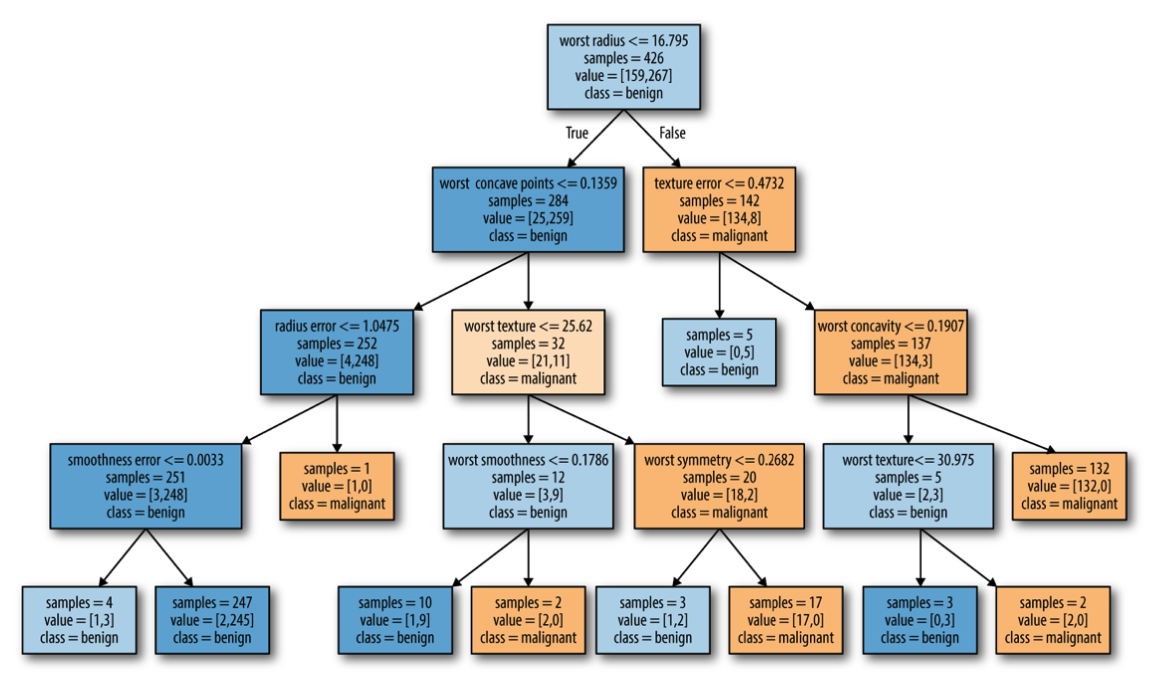
\includegraphics[scale=0.35]{decision_tree.png}
    \centering
    \caption{Visualização de uma Árvose de Decisão para um \textit{dataset} de câncer de mama \cite{muller2016introduction}.}
    \label{fig:9}
\end{figure}

\paragraph{} Por outro lado, uma desvantagem eminente é a tendência \textit{overfitting} e a baixa capacidade de generalização, que podem ser mitigados através de um algoritmo derivado chamado \textit{Random Forest}.


\subsubsection*{\textit{Random Forest}}

\paragraph{} Um dos modelos mais utilizado atualmente, o algoritmo \textit{Random Forest}\footnote{Em português: Floresta Aleatória.} é a combinação de diversas Árvores de Decisão ligeiramente diferentes entre si \cite{muller2016introduction}. A ideia é que apesar da tendência de \textit{overfitting} existente, a média dos resultados de cada árvore tende a diminuir esse fator. Além dos parâmetros responsáveis por configurar as árvores individualmente, este modelo também precisa no número de árvores que serão utilizadas.

\paragraph{} Normalmente é preferível utilizar \textit{Random Forests} ao invés de Árvores de Decisão, salvo casos em que o entendimento e a visualização clara do modelo se torna um fator importante, o que difícil de ser analisado quando existem muitras árvores. É possível compensar o aumento do tempo de processamente envolvido na criação deste modelo com paralelização em núcleos de processamento da CPU\footnote{Do inglês: \textit{Central Process Unit}.}.

\section{Considerações para Análise de Resultados}

\subsection{Índice de Sharpe}

\paragraph{} Criado pelo americano William F. Sharpe em 1966 e revisado em 1994, o Índice de Sharpe\footnote{Também conhecido como \textit{Sharpe Index}, \textit{Sharpe Ratio} ou até \textit{Sharpe Measure}.} tem como objetivo medir a performance de um investimento em relação a sua volatilidade, levando também em consideração o rendimento e a volatilidade de um investimento relativamente livre de risco (e.g., título público) \cite{sharpe1998sharpe}. Seja \begin{math}R_a\end{math} o retorno do investimento alvo, \begin{math}R_b\end{math} o retorno do investimento livre de risco e \begin{math}\sigma_a\end{math} seu respectivo desvio padrão, pode-se calcular o Índice de Sharpe através da Equação \ref{eq:1}.

\begin{equation} \label{eq:1}
    S_a = \frac{E[R_a - R_b]}{\sigma_a}
\end{equation}

\subsection{Índice de Sortino}

\paragraph{} O Índice de Sortino, criado pelo americano Frank Sortino \cite{rollinger2013sortino} é uma variante do Índice de Sharpe que considera o desvio padrão apenas dos rendimentos abaixo da média. As Equações \ref{eq:5} e \ref{eq:6} mostram seu cálculo, onde assim como no Índice de Sharpe, \begin{math}R_a\end{math} é o retorno do investimento alvo, \begin{math}R_b\end{math} é o retorno do investimento livre de risco e \begin{math}\sigma_a\end{math} seu respectivo desvio padrão. Considere também \begin{math}X_i\end{math} o i-ésimo retorno e \begin{math}T\end{math} o retorno do investimento.

\begin{equation} \label{eq:5}
    S_a = \frac{E[R_a - R_b]}{\sigma_a}
\end{equation}

\begin{equation} \label{eq:6}
    \sigma_a = \sqrt{ \frac{1}{N} \sum_{i=1}^{N} (Min(0, X_i-T))^2}
\end{equation}

\subsection{Correlação de Spearman}

\paragraph{} A Correlação de Postos de Spearman ou simplesmente Correlação de Spearman for criada pelo psicólogo inglês Charles Edward Spearman e revelada em 1904 \cite{spearman1961proof}. Em resumo, a Correlação avalia o grau de proximidade que duas variáveis aleatórias possuem em relação a uma função monotônica. Matematicamente, é o mesmo que a correlação de Pearson aplicada aos postos\footnote{Classificação ordenada das amostras em escala ordinal. Do inglês: \textit{ranks}.} das duas variáveis envolvidas.

\paragraph{} Para duas variáveis aleatórias \begin{math}X_i\end{math} e \begin{math}Y_i\end{math}, são criados os postos \begin{math}rgX_i\end{math} e \begin{math}rgY_i\end{math} para as N amostras presentes. Existem duas formas de se calcular o coeficiente: a primeira, mostrada pela Equação \ref{eq:7}, é para o caso em que há apenas postos inteiros distintos, sem presença de nós (i.e., valores iguais em cada uma das variáveis); já a segunda, ilustrada pela Equação \ref{eq:8}, é para o caso em que há presença de nós.

\begin{equation} \label{eq:7}
    \rho_s = 1 - \frac{6\sum_{i=1}^{N}d_i^2}{N(N^2-1)}
\end{equation}

\begin{equation} \label{eq:8}
    \rho_s = \rho_{rgX, rgY} = \frac{cov(rgX, rgY)}{\sigma_{rgX}, \sigma_{rgY}}
\end{equation}

\paragraph{} Na Equação \ref{eq:7}, \begin{math}d_i\end{math} é diferença entre os dois postos de cada variáveis aleatória, mostrado através da Equação \ref{eq:9}.

\begin{equation} \label{eq:9}
    d_i = rgX_i - rgY_i
\end{equation}

\paragraph{} Um exemplo prático do cálculo da correlação pode ser mostrado a partir da Tabela \ref{tab:1}, onde são ilustradas amostras para duas variáveis aleatórias \begin{math}X\end{math} e \begin{math}Y\end{math}. A Tabela \ref{tab:2} acrescenta a informação dos postos \begin{math}rgX\end{math} e \begin{math}rgY\end{math}, que ordenam as amostram em ordem decrescente. Observa-se em \begin{math}rgX\end{math} a presença de dois postos com valores de \begin{math}6.5\end{math}, causados pelo nó em \begin{math}X\end{math} de dois valores repetidos (\begin{math}61\end{math}). Neste caso, a regra é a escolha valor médio dos postos que seriam ocupados, no caso 6 e 7.

\begin{table}[h!]
    \begin{center}
        \begin{tabular}{ c|cccccccccc }
            & 1 & 2 & 3 & 4 & 5 & 6 & 7 & 8 & 9 & 10 \\
            \hline
            X & 56 & 75 & 45 & 71 & 61 & 64 & 58 & 80 & 76 & 61 \\
            Y & 66 & 70 & 40 & 60 & 65 & 56 & 59 & 77 & 67 & 63 \\
        \end{tabular}
        \caption{Amostras das variáveis aleatórias X e Y}
        \label{tab:1}
    \end{center}
\end{table}

\begin{table}[h!]
    \begin{center}
        \begin{tabular}{ c|cccccccccc }
            & 1 & 2 & 3 & 4 & 5 & 6 & 7 & 8 & 9 & 10 \\
            \hline
            X & 56 & 75 & 45 & 71 & 61 & 64 & 58 & 80 & 76 & 61 \\
            Y & 66 & 70 & 40 & 60 & 65 & 56 & 59 & 77 & 67 & 63 \\
            \hline
            rgX & 9 & 3 & 10 & 4 & \textbf{6.5} & 5 & 8 & 1 & 2 & \textbf{6.5} \\
            rgY & 4 & 2 & 10 & 7 & 5 & 9 & 8 & 1 & 3 & 6 \\
        \end{tabular}
        \caption{Postos rgX e rgY}
        \label{tab:2}
    \end{center}
\end{table}

\paragraph{} Após o cálculo dos postos, deve-se utilizar a Equação \ref{eq:8}, encontrado o valor 0.6687.

\section{Trabalhos Relacionados}

\paragraph{} Tendo em vista o conflito de interesses existente por trás de trabalhos de cujo tema está relacionado à previsibilidade do mercado financeiro, pode-se questionar se as estratégias mais promissoras de fato são encontradas em domínio público. Isso ocorre pois a democratização de uma estratégia lucrativa poderia implicar na redução das lucratividades individuais, especialmente se for utilizada em escala.

\paragraph{} Segundo KIM \cite{kim2010electronic}, somente a partir dos anos 80 que as corretoras começaram a utilizar protocolos de comunicação eletrônica para substituir a corretagem por voz. Essa inovação permitiu o desenvolvimento do Algorithmic Trading, que é a automatização da tomada de decisões de estratégias por um computador capaz de enviar ordens de compra e venda diretamente ao mercado.

\paragraph{} Para efeito de simplificação, os modelos de AT aplicados ao mercado financeiro serão agrupados em três metodologias centrais: modelos baseados em indicadores técnicos; modelos baseados em processos estocásticos; e modelos baseados em aprendizado de máquina.


\subsection{Modelos Baseados em Indicadores Técnicos}

\paragraph{} Este tipo de abordagem utiliza informações derivadas da série temporal de preços para criar uma combinação de indicadores que possuam algum poder de previsibilidade da tendência de mercado. Quando comparada aos outros tipos, é a metodologia mais simples e democrática, uma vez que pessoas com pouco ou nenhum conhecimento sobre estatística e inteligência artificial podem operar em estratégias próprias.

\paragraph{} Diversos \textit{traders}\footnote{Em português: negociantes. Pessoas que compram e vendem bens, moedas ou ações com o objetivo de lucrar, mas não necessariamente com foco em investimento, podendo até assumir um viés especulativo.} e investidores utilizam este tipo de abordagem. Dentre eles podemos citar MORAES \cite{moraes2007se}, de cujas contribuições servirão como base neste trabalho para um aperfeiçoamento via aprendizado de máquina.


\subsection{Modelos Baseados em Processos Estocásticos}

\paragraph{} De acordo com GODFREY \cite{godfrey1964random}, a hipótese de que a flutuação de preços no mercado de ações poderia ser explicada por uma Random Walk\footnote{Processo aleatório definido pela equação \begin{math}y_t = y_{t-1} + X\end{math}, onde X é uma variável aleatória e \(y\) é a variável resultante.} foi feita por BACHELIER \cite{bachelier1900theorie}. A partir da década de 60, muitos trabalhos acadêmicos foram realizados nessa linha na tentativa de entender o comportamento e a previsibilidade do mercado \cite{fama1970efficient, solnik1973note, cooper1982world}, assim como estratégias \cite{malkiel2019random}. Nota-se que até hoje utiliza-se Random Walks para testar a hipótese de eficiência de mercados \cite{said2015efficiency}.

\paragraph{} Outra abordagem utilizada são os Modelos Ocultos de Markov (do inglês Hidden Markov Model, ou HMM) \cite{rabiner1989tutorial}. Uma Cadeia de Markov é um processo estocástico que modela um sistema por meio de uma sequência finita de estados. A mudança ou a permanência em cada estado é determinada por probabilidades que dependem somente do estado atual. Em uma Cadeia de Markov, pressupõe-se que seus estados sejam observáveis, o que para algumas aplicações, pode não ser verdade. Nesse sentido surge o modelo HMM, que busca aprender sobre um processo não observável (oculto) a partir de um processo observável.

\paragraph{} Em sua pesquisa, JADHAV et al \cite{jadhav2021forecasting} utiliza um modelo HMM para previsão do preço de fechamento do dia seguinte para ações FAANG\footnote{Facebook, Amazon, Apple, Netflix, Google.}. A partir da série histórica de preços OHLC\footnote{Open, High, Low, Close. Em português: Abertura, Máximo, Mínimo, Fechamento.}, seu modelo atinge uma eficiência de 97\%-99\%, calculado a partir do erro percentual absoluto médio\footnote{Mean Absolute Percentage Error (MAPE): \begin{math} \frac{1}{N}\sum_{i=1}^{N} \frac{|Predicted(i)-Actual(i)|}{Actual(i)} \end{math}}.

\paragraph{} Uma outra aplicação de modelos HMM é dada por DE ANGELIS et al \cite{de2013dynamic}, que criou uma metodologia a partir de índices da bolsa americana capaz de identificar períodos estáveis e instáveis (i.e. crises econômicas), assim como as probabilidades de transição entre um estado e o outro.

\paragraph{} Por fim, pode-ser mencionar o uso de modelos ARCH\footnote{Em português: Heteroscedasticidade Condicional Auto-regressiva.} (Autoregressive Conditional Heteroskedasticity). A ideia central está na modelagem de uma variância condicional, ou seja, que muda de acordo o instante da série \cite{enders2008applied}. Essa característica se faz muito útil em séries que possuem períodos de alta volatilidade se alternando com períodos de baixa volatilidade. Para um modelo genérico ARCH(q), seja \begin{math}\epsilon_t\end{math} o erro (resíduo) no instante t e \begin{math}\alpha_0\end{math} um ruído branco, pode-se descrever a variância condicional de acordo com a Equação \ref{eq:4}.

\begin{equation} \label{eq:4}
\sigma_t^2 = \alpha_0 + \sum_{i=1}^{q} \alpha_i\epsilon_{t-1}^{2}
\end{equation}

\paragraph{} O modelo ARCH foi proposto por ENGLE em 1982 para estimar a variância da inflação do Reino Unido \cite{engle1982autoregressive}. A partir daí, várias derivações surgiram, como por exemplo: GARCH \footnote{Generalised ARCH.} por BOLLERSLEV \cite{bollerslev1986generalized} em 1986, EGARCH \footnote{Exponential Generalised ARCH.} por NELSON em 1991, NGARCH \footnote{Non-linear Generalised ARCH.} por HIGGINS e BERA\cite{higgins1992class} em 1992, TGARCH \footnote{Threshold Generalised ARCH.} por ZAKOIAN e RABEMANANJARA \cite{rabemananjara1993threshold} em 1993, dentre outros. Alguns dos modelos da família ARCH podem ser encontrados nos trabalhos de FRANSES e DIJK \cite{franses1996forecasting}, de MARCUCCI \cite{marcucci2005forecasting} e de ALBERG et al \cite{alberg2008estimating}.


\subsection{Modelos Baseados em Aprendizado de Máquina}

\paragraph{} Existem registros de estudos sobre inteligência artificial aplicados ao mercado financeiro por volta da década de 70 \cite{felsen1975artificial}, porém ainda em um estágio embrionário devido às dificuldades de processamento computacional e de acesso a dados na época. Por ser uma área de estudo extremamente dependente de ambas as questões, conforme elas foram evoluindo, mais trabalhos puderam ser realizados sobre o tema.

\paragraph{} NTI et al \cite{nti2020systematic} relata que dos 122 trabalhos mais relevantes publicados entre 2007 e 2018 com o tema de predição do mercado financeiro usando ML, 66\% são baseados em AT, 23\% são baseados em AF e 11\% usam análises mistas. Além disso, os algoritmos mais utilizados são ANN\footnote{Em português: Redes Neurais Artificiais.} (\textit{Artificial Neural Networks}) e SVM\footnote{Em português: Máquina de Vetor de Suporte.} (\textit{Support Vector Machine}).

\paragraph{} De forma semelhante, GANDHMAL e KUMAR \cite{gandhmal2019systematic} verificaram que a partir de uma análise detalhada de 50 trabalhos com o tema de predição do mercado financeiro, os algoritmos que mais costumam trazer resultados efetivos são ANN e técnicas baseadas em lógica \textit{Fuzzy}\footnote{Em português: Difuso.}

\paragraph{} É possível encontrar também modelos híbridos, com uma combinação de GARCH com ANN feita por BILDIRCI e ERSIN \cite{bildirici2009improving}.